\documentclass[a4paper, 14pt]{extreport}
\usepackage[T2A]{fontenc}
\usepackage[utf8]{inputenc}
\usepackage[english, russian]{babel}
\usepackage{indentfirst}
\usepackage{setspace}
\usepackage{titlesec}
\usepackage{subcaption}
\usepackage{hyperref}
\usepackage{graphicx}
\usepackage[left=2.5cm, right=1.5cm, top=2.0cm, bottom=2.0cm]{geometry}

\graphicspath{{images/}}
\renewcommand{\rmdefault}{ftm}

\titleformat{\chapter}
    {\centering\normalsize}
    {\thechapter}
    {8pt}{\MakeUppercase}
\titleformat{\section}
    {\centering\normalsize}
    {\thesection}
    {1em}{}
\titleformat{\subsection}
    {\centering\normalsize}
    {\thesubsection}
    {1em}{}
\titlespacing*{\chapter}{0pt}{-30pt}{8pt}
\titlespacing*{\section}{\parindent}{*4}{*4}
\titlespacing*{\subsection}{\parindent}{*4}{*4}

\begin{document}
    \begin{titlepage}
        \begin{center}
            Министерство образования и науки РФ \\
            Государственное образовательное учреждение\\
            Высшего профессионального образования\\
            <<Волгоградский государственный технический университет>>\\
            Кафедра <<САПР~и~ПК>>
        \end{center}
        \vspace{2.0cm}
        \begin{center}
            \large \textbf{ОТЧЁТ} \\
            по педагогической практике
        \end{center}
        \begin{flushleft}
            Студента\\
            Фамилия \underline{Голубева\hspace{3.1cm}} 
            Имя \underline{Алексея\hspace{2.1cm}}\\
            Отчество \underline{Владимировича\hspace{1.6cm}}\\
            Факультет \underline{ФЭВТ\hspace{3.45cm}} курс \underline{1\hspace{1.5cm}} 
            группа \underline{САПР-1.1п\hspace{1.9cm}}\\
        \end{flushleft}
        \vspace{1.0cm}
        \noindentТема работы: \underline{\hspace{10cm}}
        \vspace{2.0cm}
        \begin{flushleft}
            РУКОВОДИТЕЛЬ\\
            Кафедра \underline{САПР~и~ПК\hspace{2.4cm}} Должность \underline{профессор\hspace{2.8cm}} \\
            Фамилия \underline{Кравец\hspace{3.3cm}} Имя \underline{Алла\hspace{5.5cm}}\\
            Отчество \underline{Григорьевна\hspace{2.2cm}}
        \end{flushleft}
        \vspace{1.5cm}
        \begin{flushright}
            <<\underline{\hspace{1.0cm}}>>\underline{\hspace{4.0cm}} \the\year г.
        \end{flushright}
        \vspace{\fill}
        \begin{center}
            Волгоград \the\year
        \end{center}
    \end{titlepage}
    \tableofcontents
    \onehalfspacing
    \chapter{Описание методических указаний к лабораторной работе}
    OpenStreetMap~--- некомерческий веб-картографический проект, который
    создает и предоставляет свободные географические данные. Он также
    представляет возможность создавать и редактировать карты всего мира
    любому пользователю.

    Leaflet является современным проектом с открытым исходным кодом~--
    библиотека, написанная на JavaScript для отображения мобильных
    интерактивных карт. Библиотека имеет все функции, которые могут
    понадобиться большинству разработчиков для отображения веб-карт.
    Разработана с упором на простоту и производительность, а также для удобного
    использования в любых проектах. Функциональность библиотеки может быть
    расширена с помощью огромного количества плагинов, имеющие хорошо
    документированный и простой API.

    Цель методических указаний~-- ознакомить студента с технологией
    OpenStreetMap и научить основам работы с библиотекой Leaflet.

    После выполнения лабораторной работы студент получит:
    \begin{itemize}
        \item представление о технологии OpenStreetMap;
        \item базовые навыки работы с библиотекой Leaflet;
        \item повышение навыка работы с языком программирования javascript;
        \item знания о работе с картографическим сервисом.
    \end{itemize}
    
    Разработанные методические указания позволят студенту разобраться с
    современными тенденциями в веб-картографии и использовать разработанные
    технологические инструменты для собственных нужд.  

    В каждом из разделов подробно описана та или иная функциональная
    возможность технологии OpenStreetMap и библиотеки для рендеринга веб-карты
    Leaflet.

    \chapter{Сбор информации}
    Информация по проекту OpenStreetMap и Leaflet была собрана из различных
    интернет источников. Самая актуальная и достоверная информация, среди
    которой: структура, примеры использования, API, плагины была
    непосредственно взята со страниц ресурсов. Дополнительная информация по
    работе, а также разъяснение некоторых тонкостей в работе были взяты со
    следующих сайтов:
    \begin{itemize}
        \item Хабрахабр -- многофункциональный сайт, представляющий собой
            смешение новостного сайта и коллективного блога, созданный для
            публикации новостей, аналитических статей, мыслей, связанных с
            информационными технологиями, бизнесом и Интернетом.\\
            \url{http://habrahabr.ru/}
        \item OpenStreetMap (OSM) -- некоммерческий веб-картографический проект
            по созданию силами сообщества участников-пользователей Интернета
            подробной свободной и бесплатной географической карты мира.\\
            \url{http://www.openstreetmap.org/}
        \item Leaflet -- современный Open-Source проектом для отображения
            мобильных интерактивных карт.\\
            \url{http://leafletjs.com/}
        \item Wikipedia -- свободная общедоступная мультиязычная
            универсальная интернет-энциклопедия, реализованная на принципах
            Вики.\\
            \url{https://ru.wikipedia.org}
    \end{itemize}
    
    К одним из основных источников информации можно причислить Хабрахабр, так
    как в его тематических блогах имеется большое количество информации
    предоставляющее подробное объяснение по тому или иному вопросу. Стоит также
    выделить хороший стиль подачи информации и подкрепление текста визуальной
    информацией.

    \chapter{Структура методических указаний}
    В структуре методических указаний были выделены следующие пункты:
    \begin{enumerate}
        \item Цель, задачи
        \item Теоретические положения
        \begin{enumerate}
            \item Технология OpenStreetMap
            \begin{enumerate}
                \item Введение
                \item Возможности
                \item Формат данных
            \end{enumerate}
            \item Библиотека Leaflet
            \begin{enumerate}
                \item Введение
                \item Возможности
            \end{enumerate}
        \item Пример выполнения лабораторной работы
        \begin{enumerate}
            \item Задача
            \item Подготовка HTML-страницы
            \item Создание карты
            \item Маркеры, круги и всплывающие сообщения
            \item Ломаная и область
        \end{enumerate}
        \item Задания на выполнение лабораторной работы
        \item Контрольные вопросы
        \item Литература
    \end{enumerate}

    \newpage

    В разделе <<Цель, задачи>> приводится цель лабораторной работы и общие
    задачи, которые студент должен сделать во время ее выполнения.

    В разделе <<Теоретические положения>> даётся общее описание технологии
    OpenStreetMap, история возникновения и развития и используемый формат
    данных. В этом же разделе даётся описание библиотеки Leaflet и ее
    возможности.

    В разделе <<Пример выполнения лабораторной работы>> студенту
    предоставляются примеры выполнения простых заданий, снабженные подробным
    описанием выполняемых действий: от подготовки HTML-страницы, до отображения
    сложных структур данных. В нём подробно рассмотрено создание интерактивных
    карт используя простой в реализации язык программирования Javascript.

    В разделе <<Задания на выполнение лабораторной работы>> представлены
    типовые задания для закрепления изученного материала лабораторной работы.

    В разделе <<Контрольные вопросы>>~-- контрольные вопросы для проверки
    теоретического минимума по данной теме.
    
    Исходный код методических указаний доступен по следующей ссылке:\\
    \url{https://github.com/vstu-cad-stuff/osm-manual}
    
    Готовые методические указания доступны по ссылке:\\
    \url{https://db.tt/wGji7HcL}

    \chapter{Скриншоты использования библиотеки Leaflet}
    \begin{figure}[ht!]
        \center
        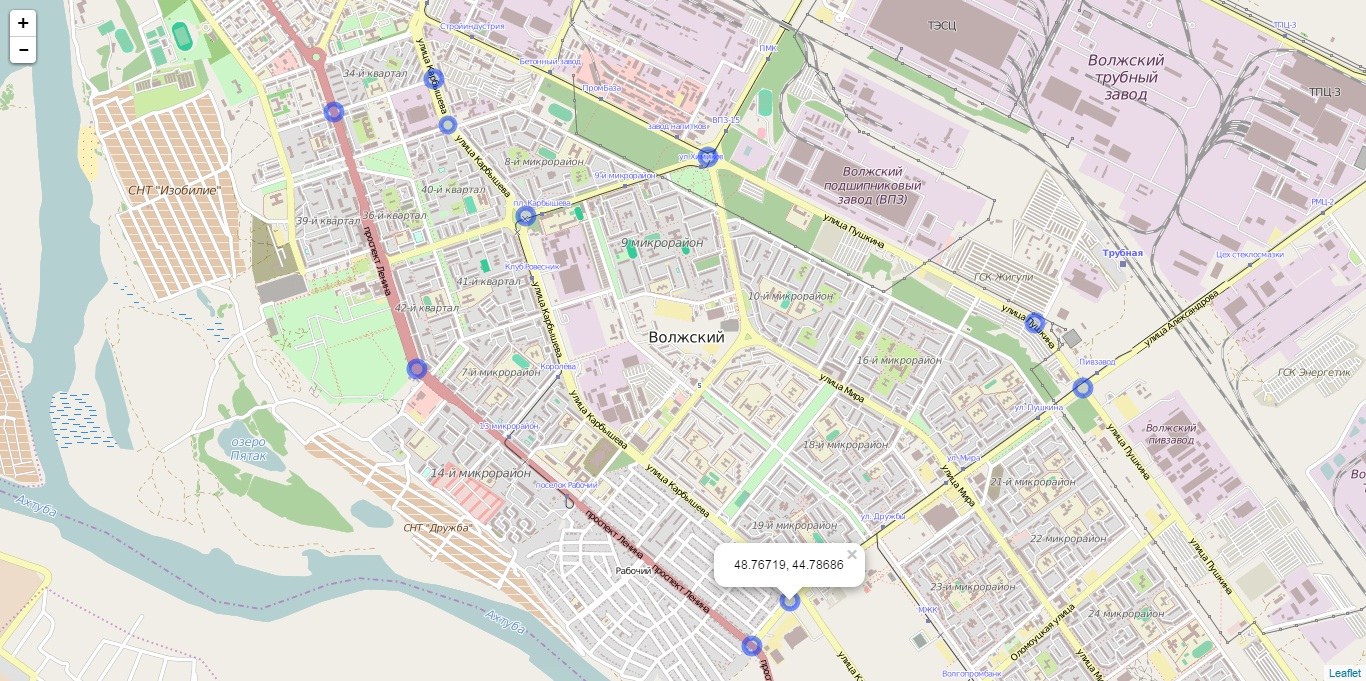
\includegraphics[width=0.9\textwidth]{e1}
        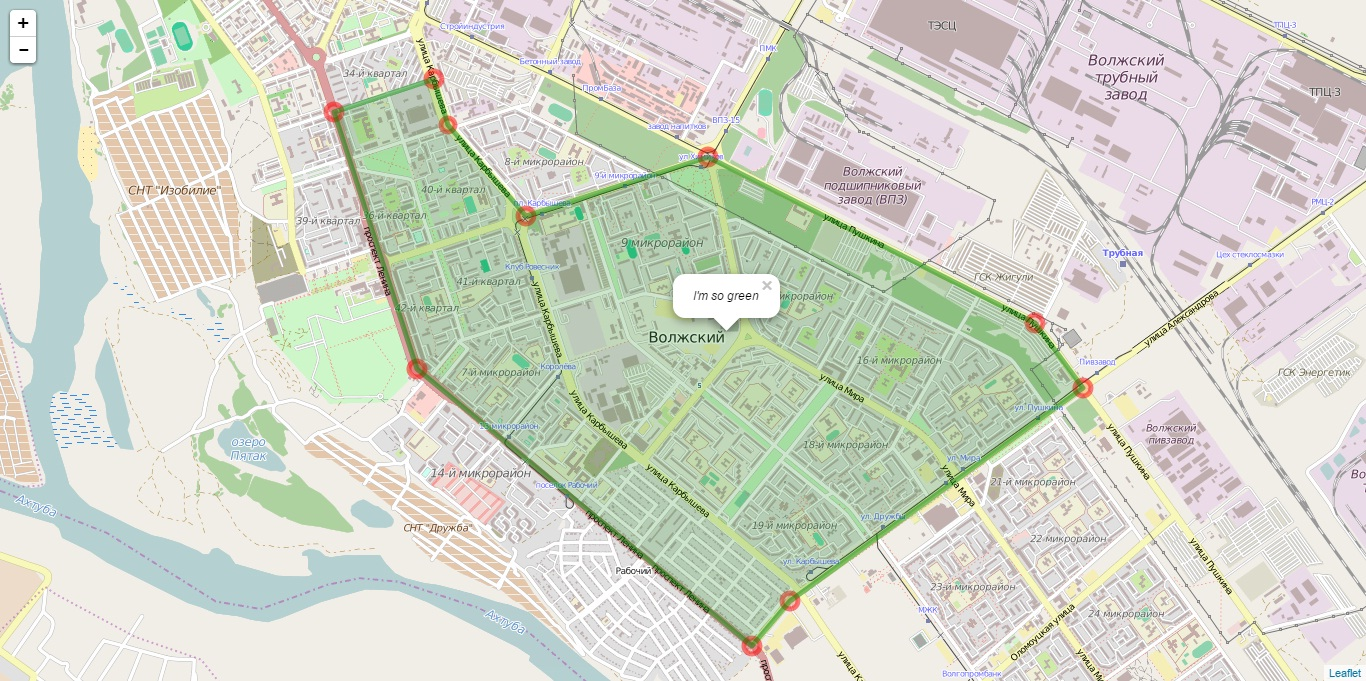
\includegraphics[width=0.9\textwidth]{e2}
        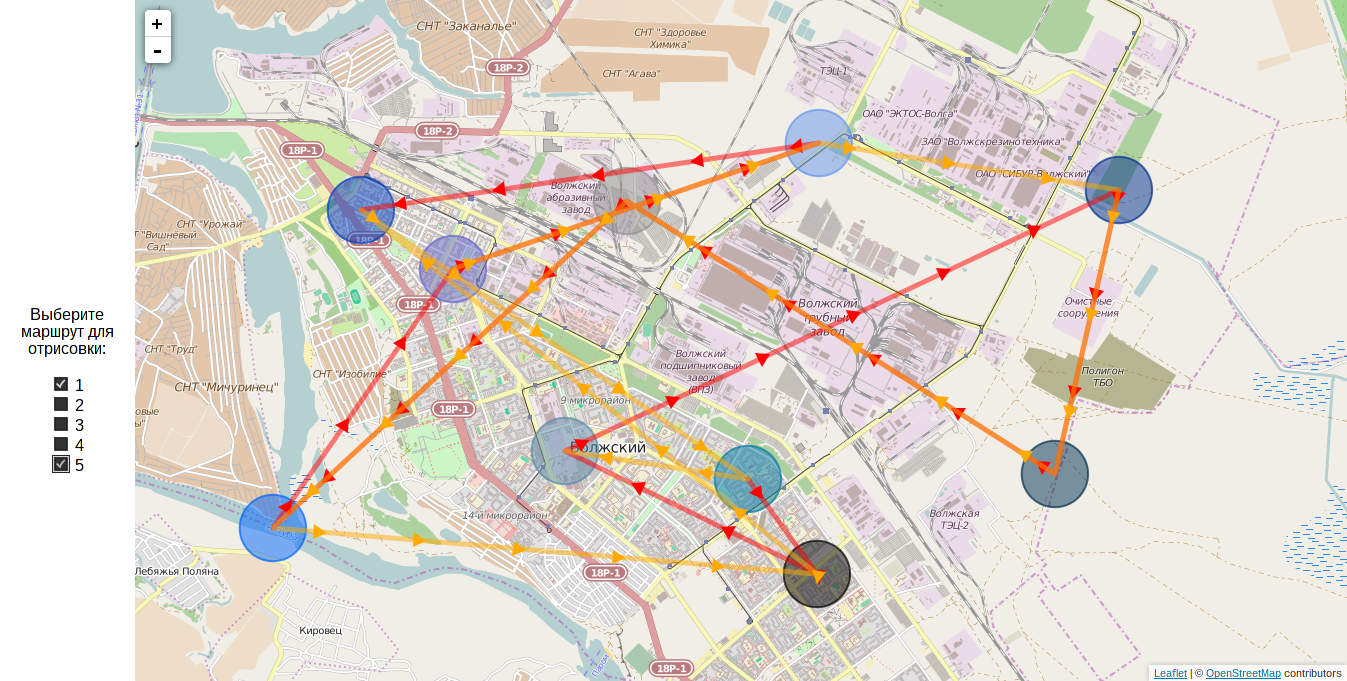
\includegraphics[width=0.9\textwidth]{e3}
    \end{figure}

    \chapter{Используемые технологии}
    Для проектирования и вёрстки были использованы следующие свободно распространяемые программные 
    продукты:
    \begin{itemize}
        \item Arch Linux -- это независимо разрабатываемый i686/x86-64 дистрибутив GNU/Linux общего 
            назначения, достаточно гибкий для выполнения любой роли.\\
            \url{https://www.archlinux.org/}
        \item \TeX -- система компьютерной вёрстки, разработанная американским профессором информатики 
            Дональдом Кнутом в целях создания компьютерной типографии.\\
            \url{http://tug.org/}
        \item \LaTeX -- набор макрорасширений системы компьютерной вёрстки TeX.\\
            \url{http://www.latex-project.org/}
        \item Sublime Text 3 -- быстрый кроссплатформенный редактор исходных текстов программ.\\
            \url{www.sublimetext.com/3}
        \item GNU Image Manipulation Program (GIMP) -- растровый графический редактор, программа для 
            создания и обработки растровой графики и частичной поддержкой работы с векторной графикой.\\
            \url{http://www.gimp.org/}
        \item Mozilla Firefox -- свободный браузер на движке Gecko, разработкой и распространением 
            которого занимается Mozilla Corporation.\\
            \url{https://www.mozilla.org/}
        \item Git -- распределённая система управления версиями файлов. Проект был создан Линусом 
            Торвальдсом для управления разработкой ядра Linux, первая версия выпущена 7 апреля 2005 года.\\
            \url{http://git-scm.com/}
        \item GitHub -- самый крупный веб-сервис для хостинга IT-проектов и их совместной разработки. 
            Основан на системе контроля версий Git и разработан на Ruby on Rails и Erlang компанией 
            GitHub, Inc.\\
            \url{https://github.com/}
    \end{itemize}
\end{document}